\documentclass[10pt,twoside,notitlepage,a4paper]{report}

\usepackage{verbatim}
\usepackage[hidelinks]{hyperref}
\usepackage{tabularx}
\usepackage{graphicx}
\usepackage{algorithm}
\usepackage{algpseudocode}
\usepackage{cleveref}
\usepackage{dirtree}
\usepackage{xcolor}
\usepackage{wrapfig}

\crefname{section}{§}{§§}
\Crefname{section}{§}{§§}

\raggedbottom                           % try to avoid widows and orphans
\sloppy
\clubpenalty1000%
\widowpenalty1000%

\addtolength{\oddsidemargin}{8mm}       % adjust margins
\addtolength{\evensidemargin}{-8mm}

\renewcommand{\baselinestretch}{1.1}    % adjust line spacing to make
% more readable

\renewcommand\DTstyle{\ttfamily\textcolor{blue}}
\renewcommand\DTstylecomment{\ttfamily\textcolor{gray}}

\setcounter{secnumdepth}{4}
\setcounter{tocdepth}{4}
\setlength{\parskip}{0.5em}%

\newcommand{\python}{\emph{Python}}
\newcommand{\unity}{\emph{Unity}}
\newcommand{\kademlia}{\emph{Kademlia}}
\newcommand{\K}{$k$}
\newcommand{\voxpop}{\emph{VoxelPopuli}}

\begin{document}
	
	\bibliographystyle{plain}
	
	\pagestyle{empty}
	
	\hfill{\LARGE \bf Samuel J. Sully}
	
	\vspace*{60mm}
	\begin{center}
		\Huge
		{\bf \voxpop:\\ A Decentralised Peer-to-Peer Voxel-Based World} \\
		\vspace*{5mm}
		Computer Science Tripos \\
		\vspace*{5mm}
		Robinson College \\
		\vspace*{5mm}
		2019-20
	\end{center}
	
	\cleardoublepage
	
	\setcounter{page}{1}
	\pagenumbering{roman}
	\pagestyle{plain}
	
	\chapter*{Proforma}
	
	{\large
		\begin{tabular}{ll}
			Name:               & \bf Samuel John Sully\\
			College:            & \bf Robinson College\\
			Project Title:      & \bf Voxel Populi: A Decentralised Peer-to-Peer\\ 
								& \bf Voxel-Based World\\
			Examination:        & \bf Computer Science Tripos -- Part II, July 2020\\
			Word Count:         & \bf \footnotemark[1]\\
			Project Originator: & \bf Samuel John Sully\\
			Supervisor:         & \bf Prof. Jon Crowcroft\\
			Director of Studies:& \bf Prof. Alan Mycroft\\
			Overseers:          & \bf Prof. Marcelo Fiore \& Dr. Amanda Prorok 
		\end{tabular}
	}
	\footnotetext[1]{This word count was computed
		by {\tt command?}
	}
	\stepcounter{footnote}
	
	\section*{Original Aims of the Project}
	My project aimed to create a peer-to-peer 3D world using a distributed hash table (DHT), namely \kademlia{}~\cite{kademlia}. I aimed to explore this decentralised, peer-to-peer approach for Massively Multiplayer Online games (MMOs) to see if such an approach is viable. This was motivated by the advantages of the decentralised approach, such as better load balancing and longevity for the game.
	
	\section*{Work Completed}
	I have completed all the work set out in my proposal, the three parts of my project are all functioning correctly. I implemented \kademlia{} with some modifications to better suit the virtual world application; I implemented the game server to run above the DHT and process the computation for a set of chunks of the world and I implemented the graphical client in \unity{} which connects to the world and allows a user to move around and interact with it. I also completed the test client which was used in the evaluation stage.
	
	\section*{Special Difficulties}
	None.
	
	\newpage
	\section*{Declaration}
	
	I, Samuel John Sully of Robinson College, being a candidate for Part II of the Computer
	Science Tripos, hereby declare that this dissertation and the work described in it are
	my own work, unaided except as may be specified below, and that the dissertation does
	not contain material that has already been used to any substantial extent for a comparable
	purpose.
	
	\bigskip
	
	\noindent I, Samuel John Sully of Robinson College, am content for my dissertation to be made available to the students and staff of the University.
	
	\cleardoublepage
	
	\tableofcontents
	
	\listoffigures
	
	\listoftables
	
	\listofalgorithms
	
	\newpage

	\cleardoublepage
	
	\setcounter{page}{1}
	\pagenumbering{arabic}
	\pagestyle{headings}
	
	\chapter{Introduction}
	
	\section{Project Summary}
	My project explores a peer-to-peer architecture for MMOs or large scale simulations. This is in contrast to the more commonly used centralised approach. My project is build upon a distributed hash table which is used to locate in the peer-to-peer network the server responsible for handling any particular part of the world.
	
	My project consists of three parts: the distributed hash table which is a modified version of the \kademlia{}~\cite{kademlia} specification; the game server which runs the computation for certain segments of the world and the \unity{} client used to interact with the world. All these have been completed in adherence to the success criteria in my project proposal, as well as the evaluation client used in the evaluation stage. The project culminated in a large scale test using Amazon Web Services.
	
	\section{Motivation}
	The Massively Multiplayer Online Game (MMO) genre is very popular\footnote{\emph{World of Warcraft} -- a popular MMO -- had 7.7 million subscribers in 2019.} in modern gaming, as an increasing proportion of the populace have access to high speed broadband the prevalence of these games continues to increase. Most of these games employ a centralised client-server mode where the creators of the MMO have a relatively small number of expensive and powerful machines which they use to handle all players.
	
	This centralised approach often requires some form of `sharding'~\cite{shard}, whereby players are separated into separate, independent instances (`shards') of the same world. Meaning that players can only interact with others connected to the same shard. The centralised approach also means that the game creators have total authoritative control over the game.
	
	An alternative approach is a decentralised, peer-to-peer approach which I explore in this project. In this approach the world is separated into segments (or `chunks') and each peer in the network is responsible for handling the load for a number of chunks. This approach implicitly performs load balancing and is highly failure tolerant, as a node failure can be dealt with by simply having another take over.
	
	This has a number of advantages over the centralised, sharded approach. One significant advantage is that the world is able to be explicitly mutable (such as the voxel-based world I have implemented), with the sharded approach if a player makes a change in one shard then we may need some way of propagating these changes to the other shards while maintaining consistency. However, in my approach there is only one server which is authoritative for the state of any part of the world so there is no need for complex consensus mechanisms.
	
	A further advantage is that the system has improved longevity. When large-scale MMOs cease to be profitable or useful for the developers, who operate the centralised servers, they often shut them down, as recently happened with the popular MMO \emph{Club Penguin}~\cite{clubpenguin} in 2017. With my approach, if we allow individuals to create their own servers to join the peer-to-peer network then, provided there exists a community dedicated to keeping the MMO running, it can continue to exist at no cost to the developers. It would even be possible to have multiple, separate networks running or even networks running modified versions of the game.
	
	\section{Related Works}
	There are very few large-scale, peer-to-peer MMOs, likely due to the security issues I will present in the evaluation chapter and due to the fact that it limits the ability for the developers to monetize the MMO post-release. However, it is possible that techniques similar to mine may be used behind the scenes on a number of large-scale MMOs.
	
	One similar piece of work is \emph{SpatialOS}~\cite{SpatialOS}, this is a platform for managing online games or simulations in the cloud. It works in a similar way to my project, by splitting up the world into segments which are administrated by separate servers. \emph{SpatialOS} is produced by the startup Improbable and is still fairly new, however, it is being used in the development of a number of games.
	
	It's worth noting also that while my implementation of \kademlia{} is custom, I used a \kademlia{} library~\cite{pykademlia} for \python{} as a reference for a fully functioning Kademlia implementation. However, this implementation uses the approach outlined in the second Kademlia paper, while my approach uses the slightly different approach from the first paper.
	
	\cleardoublepage
	\chapter{Preparation}
	
	\section{Starting Point}
	Prior to this project I had limited experience in implementing distributed systems, my knowledge on such systems mainly comes from the Part IB courses Concurrent and Distributed Systems and Computer Networking. Computer Networking introduced the concept of distributed hash tables (DHTs) which are used extensively in my project. Concurrent and Distributed Systems introduces most of the overarching principles of distributed systems, such as RPCs, which are essential in my project. Furthermore, my project relies on knowledge from a number of other courses, such as Part II Principles of Communication and Part IA Introduction to Graphics. I have some limited experience with 3D graphics from my own hobby programming as well.
	
	\section{Requirement Analysis}
	My project aims to implement a suite of software for the operation, interaction with and testing of a 3D world which is distributed over a number of peers in a peer-to-peer network. The success criteria set out in my proposal is as follows:
	
	\begin{enumerate}
		\item My DHT must adhere to the Kademlia specification. It is possible I will need to make some changes to fit the specification better to my needs and this is acceptable.
		\item The peer-to-peer node program must join the network, bootstrapping via some known node, and then will be able to participate in hosting the game world as it becomes part of the DHT.
		\item It must be possible to interact with the world using a simple 3D graphical client, which is able to place and remove voxels from the world. These changes must persist.
		\item The system must handle player moving between separate chunks (and thus, separate peers) seamlessly, with no loading screen.
		\item There must be a simple test agent which connects to and interacts with the world in some notional way to emulate the behaviour of a human user. This is for the purposes of quantitative evaluation.
	\end{enumerate}

	In addition to these criterion, the project will need to fulfil a number of other requirements:
	
	\begin{itemize}
		\item \textbf{Robustness:} the system must be very robust, handling node failures with minimal disruption to the overall system, minimising disruption to users connected to the system at a given time.
		\item \textbf{Deployment:} the implementation must run as a cloud application, being easily deployable to a large number of machines. In my testing I will be using \emph{AWS EC2} Virtual Private Servers running \emph{Ubuntu 18.04}.
		\item \textbf{Decentralisation:} the implementation must be designed to be entirely decentralised, nodes in the P2P network must be entirely equal, there must be no authoritative entity in the system.
		\item \textbf{Mutability:} the game world must emulate that of voxel-based games such as \emph{Minecraft}. As such, users must be able to edit the world and have these changes persist, users' locations must also be stored so that when they log out and back in at another time (or to a different server), they return to where they left off.
	\end{itemize}

	\section{Kademlia}
	My project is built using a DHT at its core, a DHT is a decentralised storage system based on the commonly used hash table data structure. DHTs store \textless key,value\textgreater~pairs, these are distributed among the nodes in the network, with there existing some method to partition the set of keys between the nodes, preferably in such a way that node joins or leaves require minimal changes to this partition (i.e. a node leaving does not cause the entire key-node mapping to change). The DHT maintains an \emph{overlay network} where each node maintains a set of links to other nodes in the DHT according to the topology of the network, this set of links is used in routing queries around the DHT.
	
	\subsection{XOR Metric}
	The \kademlia{} specification sets out that identifiers be $160$bit integers. Nodes IDs and keys for the DHT occupy this ID space. The notion of distance between identifiers, $d(x,y)$, is given by the bitwise XOR of the two (i.e. $d(x,y) = x \oplus y$). This is a valid metric as it obeys the following properties:
	\begin{enumerate}
		\item $d(x,x) = 0$, that is, the distance from any identifier to itself is $0$.
		\item $d(x,y) > 0$ if $x \neq y$, that is, the  distance between any two distinct identifiers is larger than $0$.
		\item $d(x,y) = d(y,x)$, that is, distances are symmetric.
		\item Distances obey  the triangle inequality, i.e. $d(x,z) \leq d(x,y) + d(y,z)$.
	\end{enumerate}
	The set of keys which a node `owns' is given by all those which are closest to its ID using the above notion of distance\footnote{This is not strictly true, actually the \K~closest nodes all store values for that key, where \K~is a parameter of the network.}.
	
	\subsection{Node State}
	Each node maintains some amount of information about other nodes in the network in order to route messages. Each node maintains a \K-bucket for each $i$ in $0 \leq i < 160$ , a \K-bucket is simply a sorted list (of length \K) of \textless IP address, UDP port, node ID\textgreater~triples of nodes between $2^i$ and $2^{i+1}$ distance away from this node. The lists are sorted by time last seen, such that the most recently seen node is at the tail of the list. This is useful later when evicting stale nodes from the \K-bucket. Note that \K~is a parameter of the network, the replication parameter.
	
	In order to populate these \K-buckets, whenever a node receivers a message from another, it looks for the appropriate \K-bucket and, if the sender is already in the \K-bucket then it is moved to the tail of the list, otherwise it is appended to the tail of the list. If the \K-bucket is full then we send a \texttt{PING} RPC to the least recently seen node, if it fails to reply then we evict it and put the new node in instead, else we discard the new node\footnote{In my implementation, the new node is added to a queue to join the \K-bucket.}.
	
	\subsection{RPCs}
	The Kademlia protocol has four RPCs: \texttt{PING}, \texttt{FIND\_NODE}, \texttt{FIND\_VALUE} and \texttt{STORE}. All other operations are built up from these four RPCs. Table \ref{tab:rpcs} details the function of each RPC. My implementation will deviate from this specification as detailed in \cref{sec:customrpc}.
	
	\begin{table}
		\begin{tabularx}{\textwidth}{| l | X |}
			\hline
			\texttt{PING} & Used to check whether a node is online, upon receiving a \texttt{PING} RPC a node will reply with its ID.\\
			\hline
			\texttt{FIND\_NODE} & Takes a $160$bit integer as argument (and identifier). When a node receives a \texttt{FIND\_NODE} RPC it returns \textless IP address, UDP port, node ID\textgreater~ triples from the \K nearest nodes to the argument identifier that it knows of.\\
			\hline
			\texttt{FIND\_VALUE} & Behaves in the same was as \texttt{FIND\_NODE} but will return a value if it possesses one for the supplied ID.\\
			\hline
			\texttt{STORE} & Takes a \textless key, value\textgreater~ pair which the receiving node stores.\\
			\hline
		\end{tabularx}
		\caption{The four \kademlia~RPCs.}
		\label{tab:rpcs}
	\end{table}
	
	\subsection{Node Lookup}
	The lookup procedure is used to locate the \K~closest nodes to a supplied identifier. The lookup procedure has one parameter, the concurrency factor $\alpha$. It proceeds as follows:
	\begin{enumerate}
		\item Find $\alpha$ closest nodes from own \K-buckets.
		\item Send \texttt{FIND\_NODE} RPCs to these $\alpha$ nodes searching for supplied identifier.
		\item Then we recursively send \texttt{FIND\_NODE} requests nodes it learned of from the results of previous steps.
		\item When an iteration of RPCs gives us no new nodes better than the current closest, we send RPCs to all of the \K~closest nodes we have not yet queried.
		\item The procedure terminates when we have received a response from all of the \K~nearest nodes.
	\end{enumerate}
	The \K~nearest nodes are returned from this procedure.
	
	\subsection{Value Lookup}
	The procedure for retrieving a value from the DHT is similar to the node lookup procedure above, replacing the \texttt{FIND\_NODE} RPCs in the above description with \texttt{FIND\_VALUE} RPCs. Instead of returning the \K~nearest nodes it will return the value found, or some notional \texttt{NULL} value if none exists.
	
	\subsection{Value Storage}
	The store value procedure consists of performing a lookup node procedure as above with the identifier being the key of the \textless key, value\textgreater~ pair to be stored. Then \texttt{STORE} RPCs with the \textless key, value\textgreater~ pair are sent to the \K~nodes returned from the lookup.
	
	\subsection{Bootstrap}
	Bootstrapping is the process by which a node joins the network. Because \kademlia{} routing information is implicitly learned through network activity we do not need an explicit \texttt{JOIN} method, we can simply use existing RPCs to join a network. All that we need is the IP, port and ID of any existing node in the network, this is the bootstrap node.
	
	The joining node, $n$, inserts the bootstrap node, $m$, into the appropriate \K-bucket and then performs a node lookup for its own ID. Finally it refreshes all its buckets which are further away than its closest neighbour. Refreshing a \K-bucket simple means picking a random ID from that bucket's range and performing a node lookup for that ID. This operation is performed automatically by each node periodically on all buckets which have not been touched in a certain amount of time\footnote{Usually 1 hour.}. By performing a lookup of itself and by refreshing those \K-buckets we have ensured that this node has been inserted into the routing tables of a number of other nodes.
	
	\section{Game Server}
	The second major part of my project is the game server, for this I will use an architecture similar to that used by \emph{Minecraft} and by \emph{Valve}'s \emph{Source} engine~\cite{source}. An instance of a game server will be the authoritative dedicated host that runs the computations for a given set of chunks of the game world, a client will connect to a number of servers in order to receive the current world state and display it to the user graphically. This section of the system is purely client server, clients do not communicate among one another, instead doing so via the server(s).
	
	The server will use an approach used in both \emph{Minecraft} and \emph{Source} where the game world is simulated in discrete time steps known as `ticks'. During a tick we process any incoming packets and update the state of the world, then we send any packets to clients in order to update the world state. In these examples world state is transferred to clients using \emph{delta compression}, where, after the initial sending of the game state, we only send changes that happened since the last tick, this reduces network load.
	
	A number of further approaches could be employed by my implementation, such as compensating for latency and interpolating between ticks. However, these are beyond the scope of my investigation and are thus not a requirement for my project.

	\section{Client}
	The third major part of my project is the client, which will be used to connect to and interact with, the world. This section of the project will require some 3D graphics, thus it will draw on material from the two graphics courses in Part IA and Part IB. I will also need to implement the algorithm for locating and loading the relevant chunks into the world so that the chunks surrounding the player's current location are always loaded.
	
	For this section of the project I decided to use \unity, rather than \emph{LWJGL}, because the graphical element was simpler and as graphics is not the focus of my project this felt appropriate.
	
	\subsection{\unity}
	\unity{} is a 3D game engine which is widely used. It is fairly easy to learn yet quite powerful and expressive making it a popular tool in the modern games industry. A simple overview is all that is needed for this project. \unity{} provides us with a 3D world populated with game objects. These game objects can have \emph{components} attached to them, such as a mesh renderer (to render a 3D mesh) or light source for example. However, most importantly you are able to assign scripts as components which you can write yourself, these scripts have a number of built-in methods which \unity{} calls at particular times, most importantly we have the {\tt Start()} method, which is called upon creating the component, the {\tt Update()} method which is called each frame and the {\tt FixedUpdate()} method which is called each time the physics engine updates. These scripts have access to a powerful API allowing us to influence the game world.
	
	\section{World \& Terrain}
	The game world will be analagous to that of \emph{Minecraft}, in that it will consist of voxels (i.e. blocks) arranged in a 3D grid. An example of \emph{Minecraft}'s terrain can be seen in figure \ref{fig:minecraft}. The \emph{Minecraft} world is broken into `chunks' each $16\times16\times256$ blocks, then each chunk is simply a 3D array of block data.
	\begin{figure}
		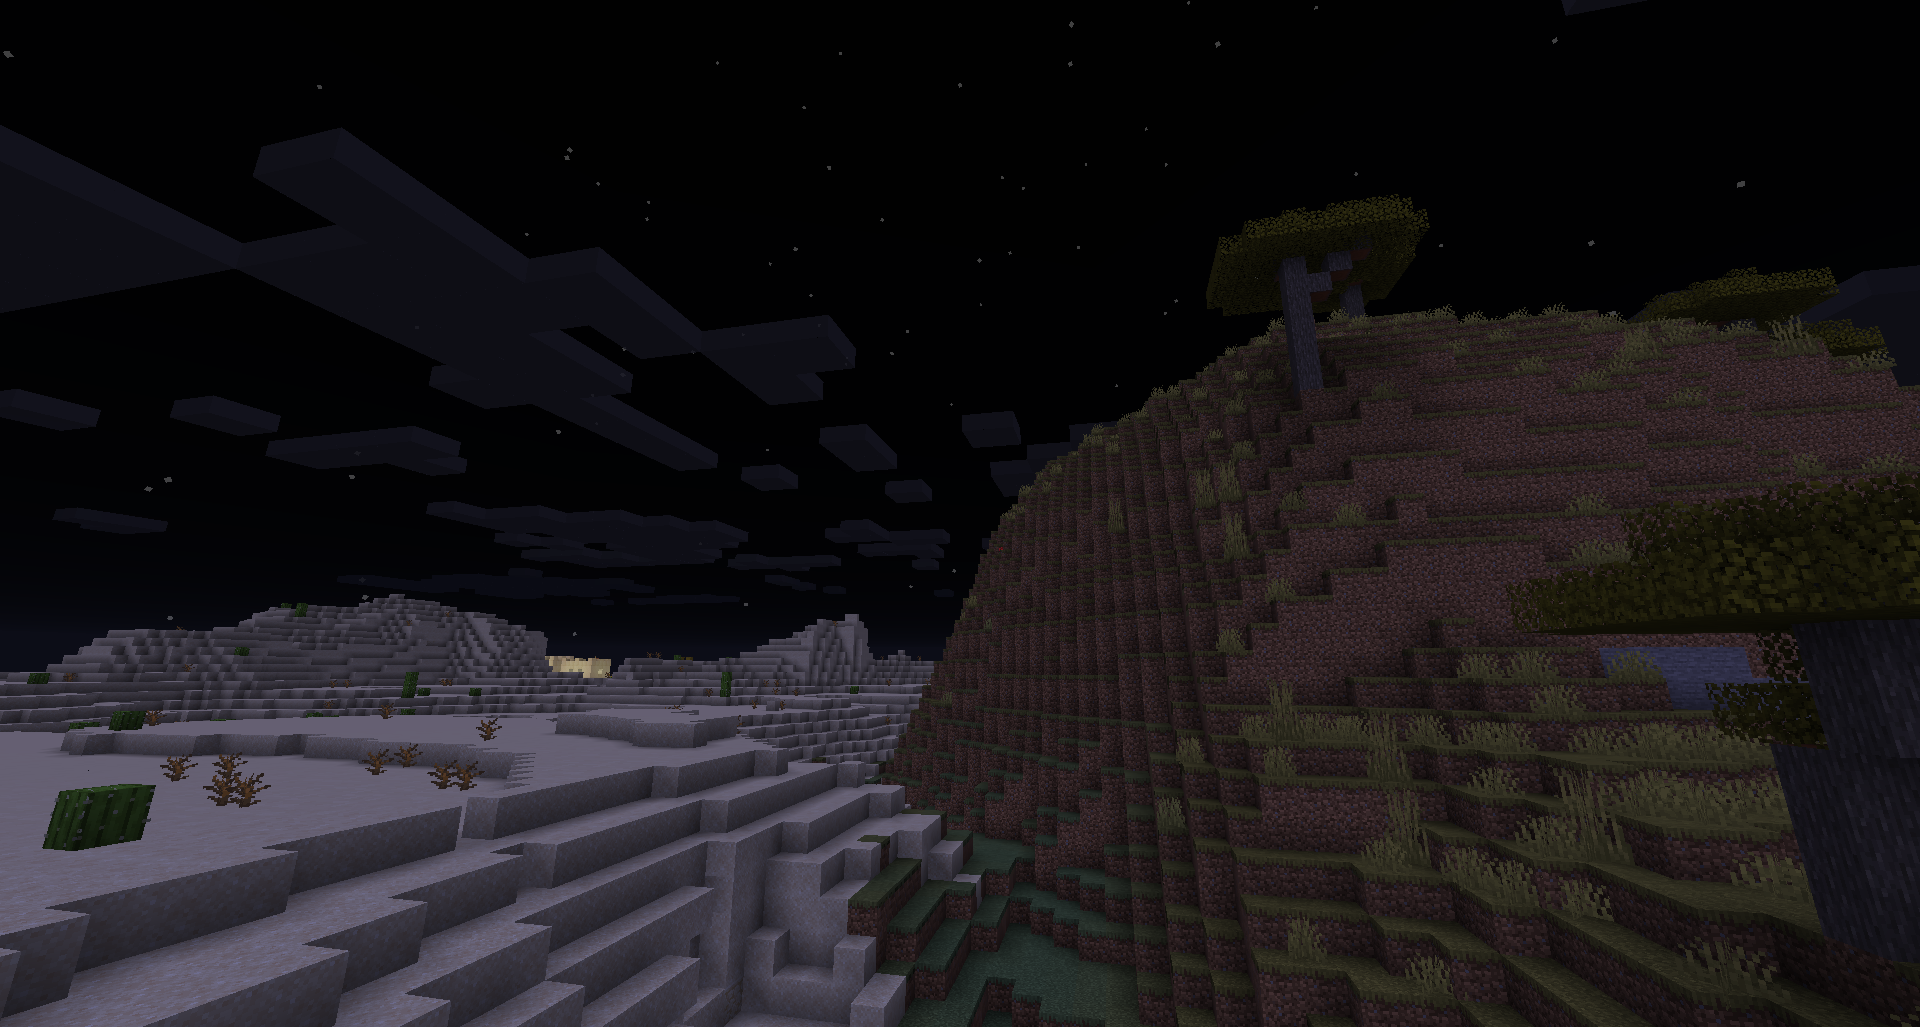
\includegraphics[width=\textwidth]{minecraft.png}
		\caption{A screenshot of terrain from the game \emph{Minecraft}.}
		\label{fig:minecraft}
	\end{figure}

	The terrain in \emph{Minecraft} is generated procedurally, allowing for infinite worlds to be created on the fly. A common approach in procedurally generated video games is to use some form of coherent noise\footnote{Coherent noise simply means smooth pseudorandom noise which obeys the following properties: \begin{enumerate} \item The same input always gives the same output. \item A small change in the input will produce a large change in the output. \item A large change in the input will produce a random change in the output.\end{enumerate}} to generate a height map\footnote{Simply a 2D function or array where the value at any given point is the height of the terrain at any given point.}. I plan to use Perlin noise~\cite{perlin} (or its successor, Simplex noise~\cite{simplex}) to generate a heightmap for my world. Then I will use simple rules to assign blocks at different heights different values (i.e. grass on top, followed by dirt, followed by stone) in order to procude a \emph{Minecraft}-like world. The structure of the world into chunks allows for easy segmentation across servers as each chunk can reside on a different server, additionally, by having data represented within a chunk as a 3D array this makes editing the world simple.
	
	\section{Professional Practice}
	\subsection{Ethical Implications} %pron - persistend customisable environment
	One ethical and legal concern is that my project would give users access to a canvas within which they could, theoretically, encode any data. This could give rise to legal issues if, for example, illegal material were encoded in world data, then the server owner on who's server that data is stored could technically be in breach of the law.
	
	\subsection{Methodology}
	The project was broken up into discrete features, with a timeline planning to complete each in approximately $2-3$ weeks. Thus I followed the \emph{Agile} software development workflow. Each $2-3$ week sprint had a deliverable which could be tested independently and demonstrated. My sprint timetable outlined in the proposal was adapted as the projected moved forward and some parts of the project took more, or less, time than anticipated.
	
	
	\subsection{Tooling}
	I used the \emph{PyCharm} IDE for the development of the \kademlia{} implementation and my game server as these were both written in \python{} using version $3.8$ due to improvements made to the \emph{asyncio} library in \python{} $3.8$. For the client I used \unity{} with \emph{Microsoft Visual Studio 2017} for editing the \emph{C\#} scripts. \emph{Git} was used for version control, with code pushed to \emph{GitHub} regularly and further backed-up daily to both the SRCF\footnote{Student-Run Computing Facility.} and the MCS using a \emph{cron} job.
	
	\subsection{Documentation}
	\textbf{Pending...}	
	
	\cleardoublepage
	\chapter{Implementation}
	My project consists of three parts: the bespoke \kademlia{} implementation, the game server and the client. The system works by having the client query the \kademlia{} implementation to locate the appropriate servers for a particular part of the world, then connecting to that server and `joining' the world via that server. This is visualised in figure \ref{fig:diagram1}.
	
	\begin{figure}
		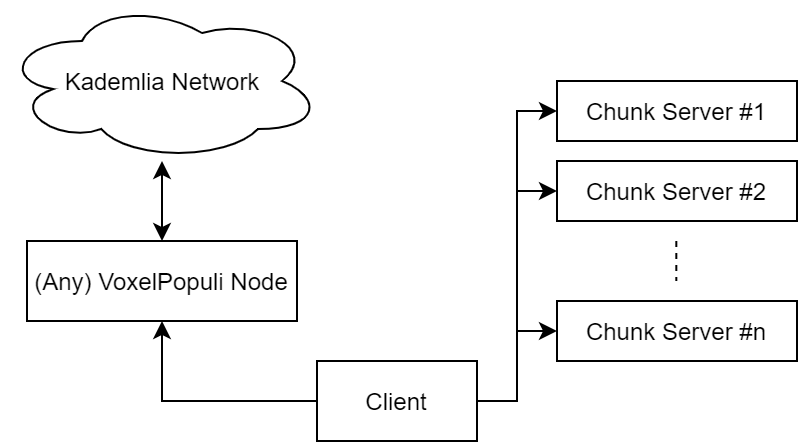
\includegraphics[width=\textwidth]{diag1.png}
		\caption{Diagram giving an overview of \voxpop{} architecture.}
		\label{fig:diagram1}
	\end{figure}
	The client needs to connect to a single node from the \voxpop{} network, which it will use as a `stepping stone' to access the whole network via. It uses this stepping stone node to query the DHT to find the \textless IP, port\textgreater~of the game servers responsible for the chunks it needs. It then initiates connections with each of these game servers in parallel, registers the player in that chunk and downloads the world data.
	
	The \voxpop{} server consists of two distinct parts, the \kademlia{} node and the game server. Thus for each node in the network there are two \emph{virtual} nodes. The \kademlia{} nodes are not visible to a client. In order to query the DHT, clients connect to any game server and initiate a special type of session specifically for DHT access. The game server then performs queries to the DHT on behalf of the client. Further details of this special session are in \cref{sec:interface}. Note that for simplicity's sake the \kademlia{} node and game server bind to the same IP address with the game server port being the \kademlia{} port incremented by $1$.
	
	\section{Kademlia}
	This section introduces my bespoke implementation of the \kademlia{} specification. A custom implementation of \kademlia{} was necessary for two main reasons:
	\begin{itemize}
		\item The project necessitated not only \texttt{PUT} and \texttt{GET} procedures but also a \texttt{GENERATE} procedure for locating the appropriate server for a particular chunk and then instructing it to generate said chunk.
		\item Two distinct types of data needed to be stored in the network. The network needed to store chunk location information (IP and port of appropriate server) and player state information in distinct areas so as not to conflate them.
	\end{itemize}
	As such, a custom implementation was devised with additional RPCs and a bespoke high-level interface with the required \texttt{PUT}, \texttt{GET} and \texttt{GENERATE} procedures.
	
	\subsection{RPC Framework}
	\label{sec:rpcframework}
	In order for \kademlia{} nodes to communicate with each other we need a method of issuing RPCs to remote machines and retrieving the results. In order to do this I used \emph{asyncio}'s \texttt{DatagramProtocol} class which is a base class for implementing protocols over UDP. This class provides overrideable methods such as \texttt{datagram\_received()} which is called when the underlying socket receives a UDP datagram. I wrote a general-purpose RPC system because at the time I was unsure how many RPCs I would need and wanted to be able to add and remove them on the fly. This proved useful when revising my \kademlia{} implementation to include the separate \texttt{STORE} and \texttt{FIND\_VALUE} RPCs.
	
	In order to implement the RPC framework I designed a \emph{JSON} format for RPC calls and responses (see table \ref{tab:rpcjson} for details). I created two function decorators in Python: \texttt{@rpc} and \texttt{@stub}. \texttt{@rpc} adds no special behaviour and simply marks that this method may be called remotely; \texttt{@stub} replaces the supplied method with a method which takes the same arguments and computes the JSON RPC string to be sent to the other machine, then sends this message and awaits a reply before returning the result (or \texttt{None} on a timeout), this process is outlined in algorithm \ref{alg:rpcstub}.
	\begin{table}
		\begin{tabularx}{\textwidth}{| l | X |}
			\hline 
			\texttt{id} & 32-bit random number to uniquely identify this RPC call.\\
			\hline
			\texttt{node} & ID of the sending node.\\
			\hline
			\texttt{call} & Boolean representing whether this is an RPC call or a response.\\
			\hline
			\texttt{rpc} & The name of the remote procedure to be called.\\
			\hline
			\texttt{args} & The list of arguments (in order) to be supplied to the remote procedure. Not present on responses.\\
			\hline
			\texttt{ret} & The return value of a remote call. Not present on calls.\\
			\hline
		\end{tabularx}
	\caption{JSON RPC specification.}
	\label{tab:rpcjson}
	\end{table}

	Upon receiving a datagram the RPC framework decodes it as a JSON string and checks whether it is a function call or a response. In the case that it is a call, the relevant function is checked to determine if it has the \texttt{@rpc} decorator (i.e. it has been marked for remote calling) and then executes it, packaging the result up as a JSON message and returning it to the sender. If it is a response, it checks if there is a pending RPC with that ID, if so it will supply the result to that RPC call, otherwise the message is discarded. This process is detailed in algorithm \ref{alg:datagram}.
	\begin{algorithm}
		\begin{algorithmic}
			\Function{rpc\_stub}{func, to\_node, args}
			\State {id $\gets$ randombits(32)}
			\State {json $\gets$ \{``id'': id, ``node'': this\_node\_id, ``call'': true, ``rpc'': func, ``args'': args\}}
			\State {store pending rpc in table}
			\State {send\_udp(json, to)}
			\State {schedule timeout}
			\State {await response OR timeout}
			\If{timed out}
			\State \Return None
			\Else
			\State {response $\gets$ get\_response(id)}
			\State \Return response
			\EndIf
			\EndFunction
		\end{algorithmic}
		\caption{RPC framework \texttt{@stub} decorator algorithm.}
		\label{alg:rpcstub}
	\end{algorithm}
	\begin{algorithm}
		\begin{algorithmic}
			\Function{datagram}{data, from}
				\State {msg $\gets$ json\_decode(data)}
				\If{msg.get(``call'')}
					\State func $\gets$ get\_function(msg.get(``RPC''))
					\If {func exists AND func has decorator \texttt{@rpc}}
						\State {res $\gets$ func(msg.get(``args''))}
						\State {json $\gets$ \{``id'': msg.get(``id''), ``node'': this\_node\_id, ``call'': false, ``rpc'': func.name, ``ret'': res\}}
						\State {send\_udp(json, from)}
					\EndIf
				\Else
					\If{rpc with id msg.get(``id'') is pending}
						\State {send msg.get(``ret'') to pending RPC calls}
					\EndIf
				\EndIf
			\EndFunction
		\end{algorithmic}
		\caption{Datagram handling in my JSON RPC framework.}
		\label{alg:datagram}
	\end{algorithm}
	
	This framework allows for the \kademlia{} specification to be implemented as described in the following sections. It allows methods to be tagged as remotely callable and allows for the creation of \emph{stub} methods which allow calling of RPCs on remote machines. This is necessary for the implementation of the \kademlia{} RPCs.
	
	\subsection{Custom RPC Specification}
	\label{sec:customrpc}
	In table \ref{tab:rpcs} I outlined the RPCs in the default \kademlia{} specification. In my implementation I have separate \texttt{STORE\_PLAYER} and \texttt{STORE\_CHUNK} RPCs as well as equivalent variants of the \texttt{FIND\_VALUE} RPCs. These replace the default \texttt{STORE} and \texttt{FIND\_VALUE} RPCs meaning we have a final specification consisting of 6 RPCs: \texttt{PING}, \texttt{FIND\_NODE}, \texttt{STORE\_PLAYER}, \texttt{STORE\_CHUNK}, \texttt{FIND\_PLAYER} and \texttt{FIND\_CHUNK}.
	
	In order to accommodate these new RPCs, the lookup procedure was made polymorphic, taking the appropriate RPC as an argument. Additionally, each node now has two separate storage tables, one for player data and one for chunk data. This implementation was preferable to the alternative of running two distinct \kademlia{} networks, as this would have significant additional overhead as two separate node states would need to be maintained for each node.
	
	\subsection{Generate Procedure}
	When a chunk is found not to exist in the network, it must be generated. In order to do this we need to first locate the server it should be generated on, then we need to check that server is up. Once we have confirmation that the server is running we send a request to the game server on that VoxelPopuli server to generate and initialise the node ready for players. If a node is not up we move to the next nearest node. Once the chunk is generated we must store the \textless IP address, port\textgreater~of the node it was generated on in the network so that in future when we look up this chunk we will find the correct server. Algorithm \ref{alg:generate} gives pseudocode of the generate procedure.
	\begin{algorithm}
		\begin{algorithmic}
			\Function{Generate}{ChunkCoordinate}
				\State $key \gets \mathrm{sha1(ChunkCoordinates)}$
				\State $nodes \gets \mathrm{lookup(key)}$
				\For{$n \in nodes$}
					\State Send generate request to game server at $<n.ip, n.port+1>$ \Comment{Game server address is that of respective \kademlia{} node with port incremented.}
					\If{Successful}
						\State Call RPC \Call{STORE\_CHUNK}{$key, <n.ip, n.port+1>$}
						\State \Return Success
					\EndIf
				\EndFor
				\State \Return Failure
			\EndFunction
		\end{algorithmic}
		\caption{Generate Procedure Pseudocode.}
		\label{alg:generate}
	\end{algorithm}
	
	\section{Game Server}
	The game server is responsible for performing the computation and maintaining the state for a number of chunks concurrently. It is also responsible for providing clients with a method of querying the DHT to locate chunks in the \voxpop{} network and to retrieve player data.
	
	\subsection{Server State}
	The game server state consists of a set of active client connections (and two queues for each connection, one for receiving and one for sending data) and the state for each of the chunks it is responsible for. Chunk state consists of the world data for that chunk, represented as a 3D array\footnote{The current size of a chunk is $32\times32\times32$ blocks.},  of integers ranging between $0-3$ to represent different voxel types (see table \ref{tab:blocks}); the set of players currently active in this chunk and their locations; a list of clients who are subscribed to updates on this chunk and $(x,y)$ -- the coordinates of this chunk in the world. Note here that a client may be connected to a single game server multiple times because it is connected to multiple of the chunks this server is responsible for.
	
	\begin{table}
		\centering
		\begin{tabularx}{0.65\textwidth}{| l | l | l | l | X |}
			\hline
			\textbf{Block Type} & Air & Stone & Grass & Dirt \\
			\hline
			\textbf{Integer Value} & 0 & 1 & 2 & 3 \\
			\hline
		\end{tabularx}
		\caption{\voxpop{} block types.}
		\label{tab:blocks}
	\end{table}
	
	Chunks are either loaded or unloaded, unloaded chunks have no connected clients and their computation (i.e. game loop) is not currently being executed. A loaded chunk has a dedicated thread for performing the game computations of the chunk, a chunk is only loaded if it has a non-zero number of connected clients and is unloaded as soon as the last client disconnects.
	
	The game server's main thread runs continuously a loop it checks if there are any new connections, in which case it will perform the handshake procedure in \cref{sec:handshake}. Furthermore, it uses \texttt{select} to get a list of sockets ready for reading or writing. Then, for each readable socket it reads all data available and adds it to the socket's buffer, if it encounters a newline character (denoting the end of a packet) it puts the packet into the receive queue associated with this socket and clears the buffer. For each writeable socket it checks if there is queued data to send and if so, attempts to send it, removing the successfully sent data from the send queue associated with that socket.
	
	\subsection{Protocol}
	\subsubsection{Handshake}
	\label{sec:handshake}
	When the server receives a new connection it waits for a JSON message from the new client, this message is decoded and it should contain a \emph{type} field. This \emph{type} field can take four different values, depending on which the server will take different actions. The possible values are:
	\begin{itemize}
		\item \textbf{``connect''} -- this means that the client wishes to connect to a chunk resident on this \voxpop{} server. There will be a field called \emph{chunk} which contains the chunk coordinates of the chunk to be connected to. The server will then perform the following:
		\begin{enumerate}
			\item Check if the relevant chunk is indeed resident and generated on this server. If not it will send a failure message to the client and return.
			\item Check whether the chunk is loaded and if not load it by starting a new chunk processing thread for this chunk (see \cref{sec:cthread}).
			\item Add this client to the chunk processing thread's client list.
		\end{enumerate}
		\item \textbf{``generate''} -- this means that the client (in fact another \voxpop{} server in this case) is requesting that a supplied chunk be generated. Again the \emph{chunk} field will be present, containing the coordinates of the chunk to be generated. The server will simply generate the chunk and add it to its set of chunks, however, it will not load it.
		\item \textbf{``dht''} -- this means that the client does not wish to use this node as a game server but instead as an access point to the DHT. In this case we launch a new, dedicated, thread to handle DHT queries, details of this thread can be found in \cref{sec:interface}.
		\item \textbf{``ping''} -- used to query whether a game server is alive, returns the \texttt{UTF-8} encoding of the string \emph{``pong''}.
	\end{itemize}
	Once the action has been completed successfully the server sends an acknowledgement to the client, informing it that the operation succeeded. Unless the connection is to be kept live (i.e. in the case of connecting to the game server (``connect'' packet) or DHT interfacing (``dht'' packet)) then the connection is closed.
	
	\subsubsection{Game}
	There are a number of messages which need to be exchanged between the client and game server. These allow the client(s) to inform the server that it has performed an action updating the world's state and allow the server to inform the client(s) of these, and other, state changes. Again these are exchanged as JSON messages of the format shown in table \ref{tab:gameprotocol}.
	\begin{table}
		\centering
		\begin{tabularx}{0.85\textwidth}{| l | l | X |}
			\hline
			Type (\texttt{int}) & Arguments (\texttt{list of floats}) & Player (\texttt{string})\\
			\hline
		\end{tabularx}
		\caption{Message format for the game server protocol.}
		\label{tab:gameprotocol}
	\end{table}

	The game server protocol consists of $6$ types of packet which are exchanged between clients and servers. The details of each packet are in table \ref{tab:gamepackets}. In order to signal the end of a packet each packet has a newline character appended to the end of its JSON representation. Packets are encoded as bytes using UTF-8 and then sent over a TCP socket between client and server.

	\begin{table}
		\begin{tabularx}{\textwidth}{| l | l | X | p{2cm} |}
			\hline
			\bf Packet Type & \bf ID & \bf Purpose & \bf Arguments \\
			\hline
			\tt PLAYER\_REGISTER & $1$ & Used by clients to inform a server that a player is entering a particular chunk. Relayed to clients to inform them they should start rendering this player. & Player location $(x,y,z)$. \\
			\hline
			\tt PLAYER\_DEREGISTER & $2$ & Used by clients to inform a server that a player has left a particular chunk. Also triggers server to save player data to DHT. Relayed by server to clients to inform they should stop rendering this player. & None. \\
			\hline
			\tt PLAYER\_MOVE & $3$ & Used by clients to update inform the server of a change in a player's location. Relayed by server to clients so they can update where the player is being displayed. & New player position $(x,y,z,\theta)$, $\theta=$ yaw. \\
			\hline
			\tt CHUNK\_DATA & $5$ & Packs entire chunk block array into packet and sends to player so they can load and display a chunk. & Flattened chunk data array. \\
			\hline
			\tt TIME & $6$ & Informs the client that the in-game time has changed, sent every tick. & Current time as minutes from midnight (accurate to second). \\
			\hline
			\tt BLOCK\_CHANGE & $7$ & Used by a client to inform the server that the world has changed, server updates state and sends updated \texttt{CHUNK\_DATA} packet to all clients. & Location of block to change and new block type. \\
			\hline
		\end{tabularx}
		\caption{List of packets types exchanged between clients and game servers.}
		\label{tab:gamepackets}
	\end{table}
	
	\subsection{Chunk Thread}
	\label{sec:cthread}
	The chunk thread performs the computation for one chunk of the world. In theory, the network should contain no more than one chunk thread for any given chunk. Meaning that clients connecting to the same chunk will always find the same server.
	
	It is important here to make a distinction between a `client' and a `player', a client is any instance of the software described in \cref{sec:client} and has an associated player with a position in the world. This client may be connected to multiple chunk threads across the network, however, the player is only resident in one of these chunks, in all the other chunks the client is simply listening to updates from this server in order to render this chunk to the user.
	
	The computation runs in a continuous loop, it pops any packets from its receive queue and performs the appropriate action as explained in table \ref{tab:gamepackets}, this may involve updating the game state and hence, sending packets to some of the clients connected. It then steps the game time and sends all players in this chunk a packet informing them of the time change. Next it checks if any player has not been heard of for a certain period of time and removes it, assuming it has gone offline.
	
	When there are no active clients for this chunk thread it will unload, saving the state and stopping the thread so as not to waste resources. This ensures that the number or chunk threads active on a given node at a particular time is kept to a minimum.
	
	\subsection{DHT Interface}
	\label{sec:interface}
	As previously explained, in order for clients to query the DHT (and thus retrieve their saved player data and the locations of chunks in the network) they must have some method to query the DHT. In order to do this they connect to a game server and perform the DHT handshake as described in \cref{sec:handshake}. This connection is then given a dedicated thread to respond to queries to the DHT. The current protocol allows a client to either get the \textless IP, port\textgreater~ for a particular chunk (the chunk is generated if does not exist in the network) or download player save data (location primarily).
	
	\subsubsection{Protocol}
	The thread process one request at a time and is not guaranteed to respond to requests issued while another request is pending. There are two packet types chunk query (type $0$) and player query (type $1$), a packet's first byte is its packet type. To query a chunk location a packet is sent consisting of a leading $0$ byte (packet type) followed by the JSON encoding of the coordinates of the chunk (as a JSON list). The server replies with the JSON list \texttt{[IP address, port]}. To query player data a packet consisting of a leading $1$ byte (packet type) followed by the JSON attribute-value pair: \texttt{\{`name':player\_name\}} where \texttt{player\_name} is the username of the player to query. The server responds with the JSON representation of the player's coordinates. If the player was not found then it returns $(0,32,0)$ (the default spawn location). Note that all the JSON strings are encoded as bytes for sending using UTF-8.
	
	\section{Client}
	\label{sec:client}
	The client is the user's entry point into the world, it renders the world (and other players) and allows the player to move around within it; it provides a basic physics simulation for realistic movement and collisions and it allows the user to make changes to the world by breaking and placing blocks. A screenshot of the client in action can be seen in fig \ref{fig:client}. The client was written in C\# using the \unity{} game engine.
	
	\begin{figure}
		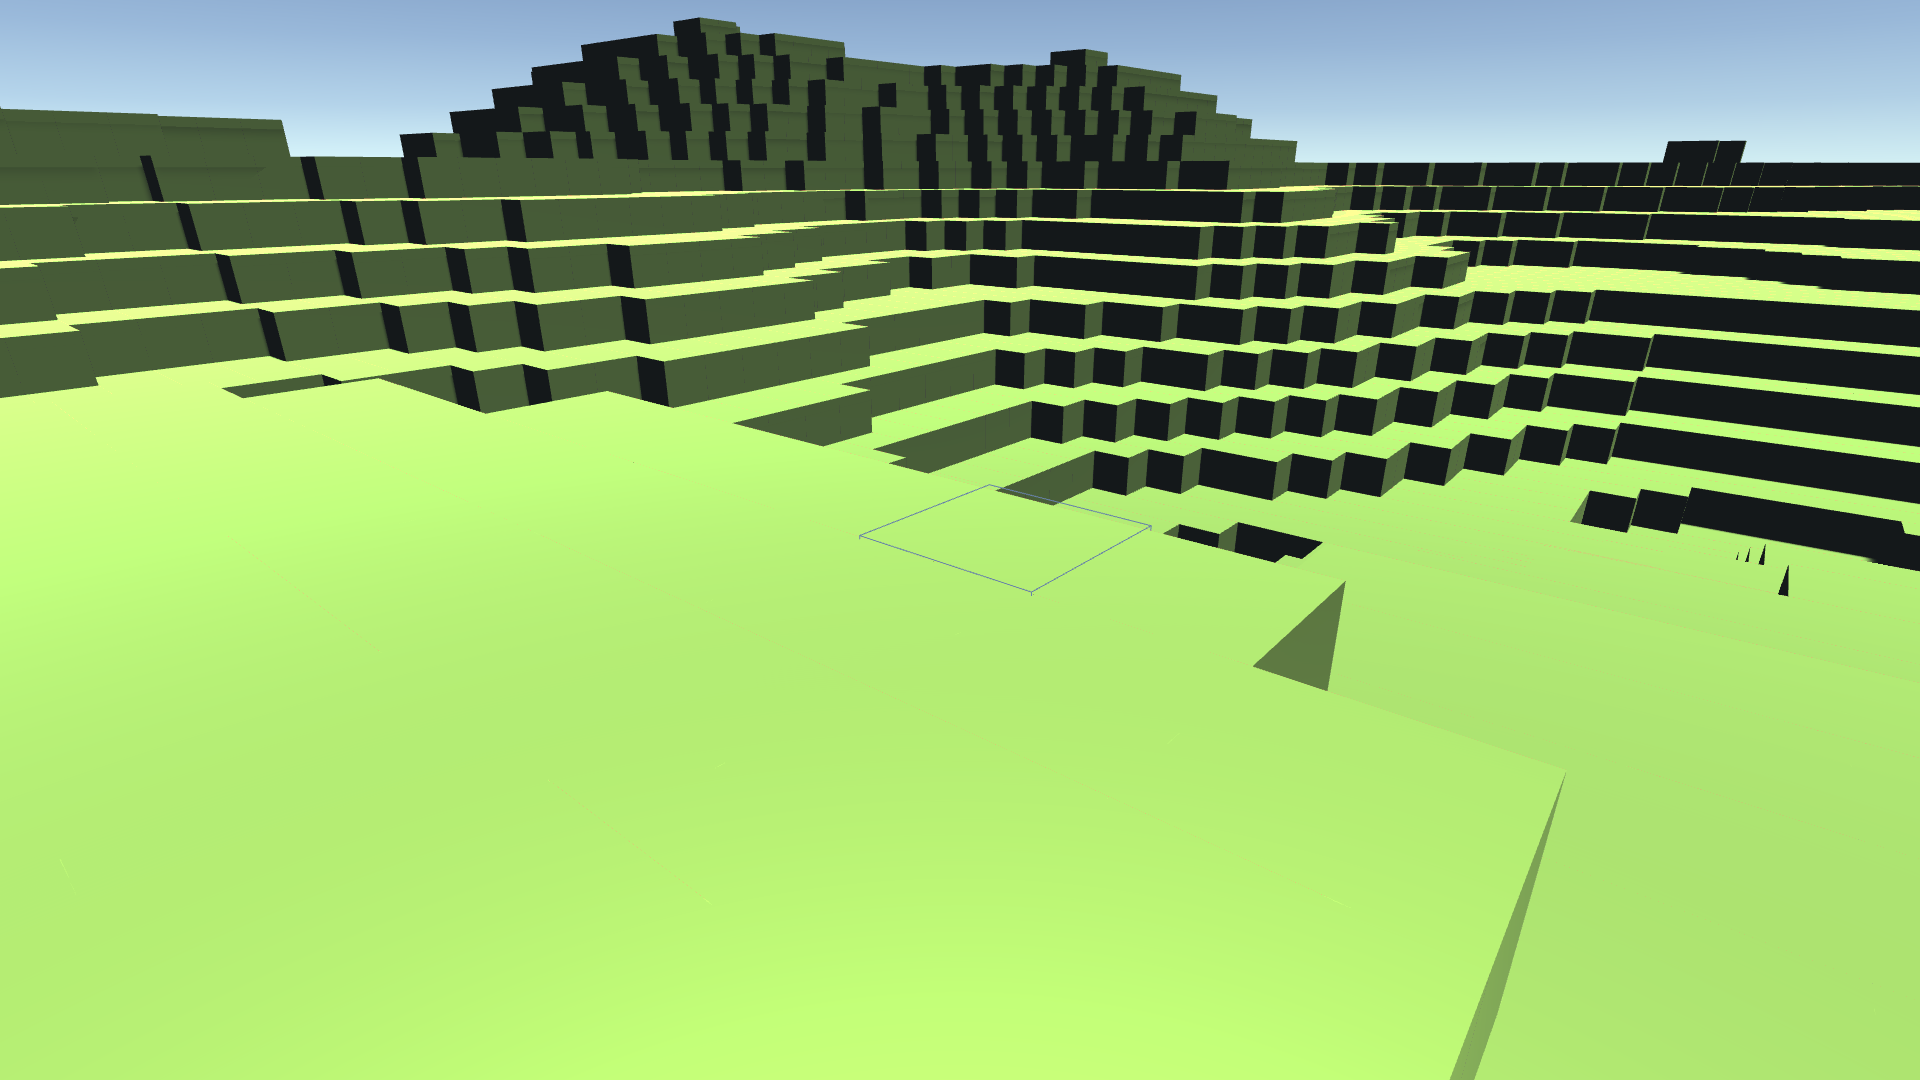
\includegraphics[width=\textwidth]{client.png}
		\caption{A screenshot of the \voxpop{} client connected to a world.}
		\label{fig:client}
	\end{figure}
	
	\subsection{Architecture} % talk about multithreading and packets -> updates
	The client operates two main threads as well as a two threads (one each for receiving and sending) for each chunk it is connected to. The two main threads exist to separate long, blocking processes from the thread rendering the world, this prevents frame rate stuttering\footnote{Where the frame rate drops briefly, causing the game to appear to momentarily freeze}. The two main threads will be referred to as the \emph{network thread} and the \emph{game thread}.
	
	\begin{table}
		\begin{tabularx}{\textwidth}{| l | X | p{3cm} |}
			\hline
			\bf Update Type & Purpose & Arguments \\
			\hline
			\tt PLAYER\_MOVE & Used by the network thread to inform the game thread that another player has moved and the object representing that player should be moved. & Player name and new location.\\
			\cline{2-2}
			\tt & Used by the game thread to inform the network thread that the player associated with this client has moved so that the network thread can relay this to the server. & \\
			\hline
			\tt LOAD\_CHUNK & Used by the network thread to make the game thread load in newly downloaded chunk data. & Chunk coordinates, block array and mesh data. (Encapsulated as a `Chunk` object.) \\
			\hline
			\tt UNLOAD\_CHUNK & Used by the network thread to make the game thread unload a chunk, removing it from the game world. & Chunk coordinates. \\
			\hline
			\tt PLAYER\_ADD & Used by the network thread to inform the game thread of a player appearing in a particular chunk, the game thread will add an object to the world to represent this player. & New player's location and name. \\
			\hline
			\tt PLAYER\_REMOVE & Used by the network thread to inform the game thread a player has left a particular chunk, the game thread removes the player from the world. & The player's name. \\
			\hline
			\tt TIME & Network thread informs the game thread a \texttt{TIME} packet has been received, the game thread will move the game's light object to reflect this. & The new time. \\
			\hline
			\tt BLOCK\_CHANGE & Used by the game thread to inform the network thread the player has broken or placed a block. & The position of the block to be updated and its new type.\\
			\hline
		\end{tabularx}
		\caption{Details of the updates exchanged between the network and game threads of the client.}
		\label{tab:updates}
	\end{table}
	
	\subsubsection{Network Thread}
	\label{sec:nthread}
	The network thread has access to send/receive queues for each chunk the client is connected to. It takes received packets from these queues and processes them ready to be sent to the game thread. Some packets require an amount of computationally intensive pre-processing before they are ready to be used by the game. For example, packets of type \texttt{CHUNK\_DATA} require a large amount of processing as the array needs to be unflattened and then the chunk's mesh data needs to be generated -- this can take $10$s of frames. This computation is performed in the network thread which has no bearing on the client's frame rate. Once any pre-processing is performed a state update is sent to the game thread which is rendering the world.
	
	The network thread also receives updates from the game thread, these updates can be player movement or block changes. Where appropriate, it converts these updates into a packet and queues these for sending to the relevant chunk's server.
	
	Finally, the network thread ensures that the correct chunks are loaded, locating and loading those which are needed and unloading those which are no longer needed. This is discussed in detail in \cref{sec:loading}. To do this is maintains a connection to a \voxpop{} node where the connection has been setup to be in DHT query mode, allowing the client to use this node to query the DHT.
	
	\subsubsection{Game Thread}
	\label{sec:gamethread}
	This is the main \unity{} thread. The part that is of interest to this project is the \texttt{update()} method in our \texttt{World} script which is executed each frame. This has access to the incoming and outgoing update queues used to exchange state updates between the network thread and the game thread. The game thread simply performs the necessary steps to make state updates received from the network thread visible to the user, and it sends updates to the network thread when the user does something which updates the state of the world.
	
	Details of the types of updates exchanged can be seen in table \ref{tab:updates}. Some of these are very similar to the packets from table \ref{tab:gamepackets} as expected. Within the game thread each player has an object to represent it (in this prototype they are simply a cube) and each chunk has an object to represent it (a 3D mesh with an associated `Chunk' object containing the block array and the mesh's data -- details of mesh data generation are in \cref{sec:mesh}).
	
	\subsection{Chunk Mesh Generation}
	\label{sec:mesh}
	In computer graphics, a \emph{mesh} is a collection of vertices, edges and faces which make up a 3D object. For each chunk we must generate a mesh from the block array in order to render the chunk to the player. In order to do this we must construct 2 arrays; firstly, we need to compute the array of vertices in the mesh, then we need the array mapping these vertices to triangles. In order to do this, for each triangle we need the indices of the 3 vertices that make up that triangle, we then add these 3 indices to the triangles array.
	
	\begin{figure}
		\centering
		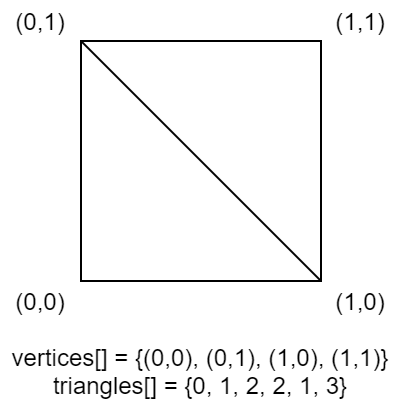
\includegraphics[width=0.5\textwidth]{diag2.png}
		\caption{A diagram of mapping between vertices and triangles for a simplified face of a cube.}
		\label{fig:mesh}
	\end{figure}
	
	In order to apply textures to the faces we also need to provide a texture coordinate (often referred to as a \emph{uv} coordinate) to each vertex. This is supplied in an array too, where the indices in the vertex array correspond to the indices of the texture coordinate of that vertex in the uv array. Once we have computed our vertex, triangle and uv arrays we can supply these to unity which will be able to generate and render the mesh for us. This process is very computationally intensive, for our chunks it involves iterating over all $32^3 = 32768$ blocks and performing $6$ iterations ($1$ per face) for each block. Pseudocode for the mesh generation algorithm is supplied in algorithm \ref{alg:mesh}, this approach is based on similar methods found in various open source voxel-based games. Figure \ref{fig:mesh} shows how a face of the cube is produced by two triangles.
	
	\begin{algorithm}
		\begin{algorithmic}
			\State blocks[][][] $\gets$ chunk block array;
			\State vertices[] $\gets$ new vec3 array;
			\State triangles[] $\gets$ new int array;
			\State uvs[] $\gets$ new vec3 array;
			\State vertex $\gets 0$;
			\For{$0 \leq x <$ \tt CHUNK\_SIZE}
				\For{$0 \leq y <$ \tt CHUNK\_SIZE}
					\For{$0 \leq z <$ \tt CHUNK\_SIZE}
						\For{each face}
							\If{blocks[x][y][z] is air OR\\ blocks[x][y][z] + faceNormal is not air}
								\State continue;
							\EndIf
							\State add vertices for this face;
							\State add uv coordinates for correct texture;
							\State triangles += [vertex+0, vertex+1, vertex+2];
							\State triangles += [vertex+2, vertex+1, vertex+3];
							\State vertex $\gets$ vertex + 4;
						\EndFor
					\EndFor
				\EndFor
			\EndFor
		\end{algorithmic}
		\caption{The mesh generation algorithm used by the client.}
		\label{alg:mesh}
	\end{algorithm}
	
	\subsection{Chunk Loading \& Unloading}
	\label{sec:loading}
	As noted in \cref{sec:nthread} the network thread is responsible for ensuring the correct chunks are loaded, it uses the DHT query connection for this purpose. The rule for determining whether a chunk should be loaded is simple: a chunk should be loaded if it is not already loaded and it is within a $3\times3$ grid of chunks centred on the player. Similarly, a chunk should be unloaded if it is outside of a $9\times9$ grid of chunks centred on the player.
	
	Each time the network thread processes a \texttt{PLAYER\_MOVE} update from the game thread it checks to see if there are any chunks to unload, if so it unloads them (i.e. ends the connection and sends a \texttt{CHUNK\_UNLOAD} update to the game thread). Then it checks if there are any chunks to load, if so it queries their locations using the DHT connection, connects to them and loads them (it only sends the \texttt{CHUNK\_LOAD} update when it receives the \texttt{CHUNK\_DATA} packet from the server for this chunk). This process is outlined in algorithm \ref{alg:load}.
	
	\begin{algorithm}
		\begin{algorithmic}
			\For{chunk $\in$ loaded}
				\If{$|\mathrm{chunk.x} - \mathrm{player.chunk.x}| \geq 5$ OR $|\mathrm{chunk.y} - \mathrm{player.chunk.y}| \geq 5$}
					\State unload(chunk);
				\EndIf
			\EndFor
			\State chunk\_position $\gets$ (player.chunk.x, player.chunk.y);
			\For{$-1 \leq i \leq 1$}
				\For{$-1 \leq j \leq 1$}
					\If{chunk at chunk\_position + $(i,j)$ is not loaded}
						\State s $\gets$ query\_chunk\_from\_dht(chunk\_position + $(i,j)$);
						\State load chunk from server s;
					\EndIf
				\EndFor
			\EndFor
		\end{algorithmic}
		\caption{Algorithm for maintaining the correct set of loaded chunks by the client.}
		\label{alg:load}
	\end{algorithm}
	
	\section{Overview}
	This section provides an overview of the project and the files contained within my repository (which are shown in figure \ref{fig:dir} shows).
	
	\begin{wrapfigure}{R}{5.5cm}
		\dirtree{%
			.1 \voxpop.
			.2 Client.
			.3 Assets.
			.4 Code.
			.5 Chunk.cs.
			.5 Constants.cs.
			.5 Controller.cs.
			.5 Network.cs.
			.5 WireFrame.cs.
			.5 World.cs.
			.4 $\dots$.
			.2 Server.
			.3 main.py.
			.3 game.
			.4 chunkthread.py.
			.4 const.py.
			.4 world.py.
			.3 kademlia.
			.4 node.py.
			.4 protocol.py.
			.4 router.py.
			.4 server.py.
			.4 storage.py.
			.3 tests.
			.4 $\dots$.
			.2 Test Client.
			.3 test\_client.py.
		}
		\caption{Directory overview of \voxpop{}.}
		\label{fig:dir}
	\end{wrapfigure}
	
	\subsection{Client}
	The client takes the form of a \unity{} project. As noted, Unity allows you to assign scripts to game objects which then have methods such as \texttt{Update()} and \texttt{Start()} which are called at the appropriate times (in these cases: each frame and when the object is created respectively).
	
	The client has $6$ files of code, $3$ of which contains scripts able to be assigned to objects. {\tt Controller.cs} is a script assigned to the player object which takes user input and moves the player, obeying physics and collisions. {\tt WireFrame.cs} is another script applied to the player object which simply renders a wire frame cube around the block the player is looking at. {\tt World.cs} is a script applied to the (initially) world object which performs the game thread actions described in \cref{sec:gamethread}.
	
	The other $3$ files contain classes and data used by the aforementioned scripts. In {\tt Chunk.cs} we have a class for chunks, these contain the chunk's block array and mesh data, and provide a number of methods for querying the contents of the chunk (such as {\tt IsSolid(Vector3 localPos)} for querying if a block is solid at position {\tt localPos} relative to the chunk). {\tt Network.cs} contains the {\tt NetworkThread} class which is used to execute the network thread as explained in \cref{sec:nthread}. Finally, {\tt Constants.cs} contains a number of constants such as the tick rate, chunk size and various pieces of data needed for mesh generation.
	
	\subsection{Server}
	The server is split into two main parts, the \kademlia{} implementation and the game server. Within the game server we have {\tt chunkthread.py} which contains the {\tt ChunkThread} class which is used to execute the chunk thread as discussed in \cref{sec:cthread}. We also have {\tt world.py} which contains classes for maintaining state about the world, namely {\tt Chunk} and {\tt Player}. We have {\tt const.py} which contains a number of important constants such as a {\tt PacketType} enumeration. Finally we have {\tt main.py} which performs the main loop of a \voxpop{} node, i.e. waiting for new connections and performing the handshake procedure from \cref{sec:handshake}. The code for the DHT interface thread (see \cref{sec:interface}) is here too.
	
	Within the \kademlia{} folder we have {\tt node.py} and {\tt storage.py} which contain simple classes to represent a \kademlia{} Node and the local storage on a node respectively. {\tt router.py} contains the \K-bucket class and routing table class. {\tt protocol.py} contains the \kademlia{} RPC implementation as well as the RPC framework outlined in \cref{sec:rpcframework}. Finally, {\tt server.py} contains the high level interface for the \kademlia{} network, allowing the following operations to be performed: {\tt run()} (initialise a node), {\tt get\_chunk()} (lookup a chunk and generate it if it does not exist), {\tt get\_player()} and {\tt save\_player()} (retrieve or save player save data), {\tt generate\_chunk()} and {\tt republish\_chunk()}.
	
	\subsection{Test Client}
	The test client is a single script which simply initialises a configurable number of dummy players and connects them to the network in random positions, it then moves them around randomly to simulate activity.
	
	\textbf{MORE ON THIS PLS SAM}
	
	\cleardoublepage
	\chapter{Evaluation}
	\section{Methodology}
	This project aims to explore the viability of using a peer-to-peer network topology for a large online world with potentially thousands of players. Unfortunately I do not have access to enough machines (and indeed players) to accurately field test the project. I shall instead be performing two main types of testing to prove the viability of \voxpop{} as a MMO engine. I will be performing local simulations using simulated players (created by my test client) to demonstrate the load that a single server experiences under different scenarios. Then I will create, using AWS, a small network of around $150$ nodes which will be populated by simulated players to prove that the system is able to perform at scale.
	
	I will also be testing the system by subjecting it to failure modes such as node failure, and demonstrating that it continues to operate correctly in these scenarios. I will perform a high-level analysis of the security of \voxpop{} and its susceptibility to various attacks. Additionally, I will be investigating the adherence of the \kademlia{} implementation to the specification.
	
	Finally some simple tests on the client will be performed and then I will consider the limitations that the peer-to-peer approach presents when compared to the more commonplace client-server model.
	\section{\kademlia{} Implementation}
	\section{Scalability}
		\subsection{Local Simulation}
		\subsection{Large Scale Simulation}
	\section{Security}
	\section{Client Performance}
	\section{Current Limitations}
	
	\cleardoublepage
	\chapter{Conclusion}

	\cleardoublepage
	
	\addcontentsline{toc}{chapter}{Bibliography}
	\begin{thebibliography}{9}
		\bibitem{kademlia} Maymounkov, P. and Mazières, D. Kademlia: A Peer-to-peer Information System Based on the XOR Metric. \url{https://pdos.csail.mit.edu/~petar/papers/maymounkov-kademlia-lncs.pdf}. Accessed: 2019-10-16.
		\bibitem{shard} ``Sharding'' on Wikipedia. \url{https://en.wikipedia.org/wiki/Shard_(database_architecture)}. Accessed: 2019-10-15.
		\bibitem{clubpenguin} ``Club Penguin is shutting down''. \url{https://techcrunch.com/2017/01/31/club-penguin-is-shutting-down/}. Accessed: 2019-10-15.
		\bibitem{SpatialOS} SpatialOS by Improbable. \url{https://improbable.io/spatialos}. Accessed: 2020-03-20.
		\bibitem{pykademlia} Kademlia Python Library. \url{https://github.com/bmuller/kademlia/}. Accessed: 2020-03-20.
		\bibitem{source} Source Engine Multiplayer Networking, Valve. \url{https://developer.valvesoftware.com/wiki/Source_Multiplayer_Networking}. Accessed: 25-3-2020.
		\bibitem{perlin} ``Perlin Noise'' on Wikipedia. \url{https://en.wikipedia.org/wiki/Perlin_noise}. Accessed: 2019-10-17.
		\bibitem{simplex} ``Simplex Noise'' on Wikipedia.
		\url{https://en.wikipedia.org/wiki/Simplex_noise}. Accessed: 2019-03-27.
	\end{thebibliography}
	\cleardoublepage
	
	\appendix
	
	\chapter{Proposal}
	
\end{document}